\section{Results}
\label{sec:results}

We have taken a number of departures from traditional application of the IB method and
RBC models. In the following sections, we establish convergence for our implementation
of RBF-IB, demonstrate impermeability of the RBCs, and observe typical RBC behaviors
before presenting the results of our whole blood simulations.

\subsection{Convergence study}\label{sec:convergence}

In this section, we perform a series of tests on a single perturbed RBC undergoing
relaxation. We simplify the RBC model and use only Skalak's Law. We expect the IB method
to approximate the fluid velocity at first order for thin shells, as it cannot recover
the pressure jump across the interface. We stretch the RBC by a factor of 1.1 in the $z$
direction and compress it in the $x$ direction to maintain its reference volume. We place
the cell in the center of a $16\um\times16\um\times16\um$ domain with homogeneous
Dirichlet boundary conditions in the $y$ direction and periodic boundaries elsewhere. The
fluid velocity is initially zero. The cell is then allowed to relax for $180\us$.

We use the 3-point kernel $\hat{\Dirac}_1$ derived by Roma \latin{et al.}~%
\cite{Roma:1999tx} for spreading and interpolation and the 2-stage RK method described in
Section~\ref{sec:ib} to advance the fluid velocity. Fluid grids are chosen to have $20r$
grid points per $16\um$ in each direction for $r$ from 1 to 6. On successive grids, we
compare the fluid velocity at cell centers in a regular grid of $20^3$ cells and surface
positions at 1000 surface points. For convergence of order $p$, we expect the ratio of
successive errors to satisfy
\begin{equation}
    \frac{\epsilon_r}{\epsilon_{r+1}} = \left|\frac{((r+1)/r)^p-1}{((r+2)/(r+1))^{-p}-1}\right|,
\end{equation}
which we solve numerically to determine $p$. We compute the errors in $\X$ using discrete
versions of the $L_2$ and $L_\infty$ norms,
\begin{gather}
    \|\X(\theta,\,\varphi)\|_2^2 =
    \int\limits_{\sphere} \X(\theta,\,\varphi)\cdot\X(\theta,\,\varphi) \d\qs \quad\text{and} \\
    \|\X(\theta,\,\varphi)\|_\infty^2 =
    \max_{(\theta,\,\varphi)} \X(\theta,\,\varphi)\cdot\X(\theta,\,\varphi),
\end{gather}
respectively.

Tables~\ref{tab:u-rbc-conv} and~\ref{tab:x-rbc-conv} show $L_2$ and $L_\infty$ errors in
$\u$ and $\X$ between successive grids. We observe first-order convergence, as expected.
Satisfied with the convergence of our implementation, we henceforth continue using the
Bauer spiral to discretize RBCs and use the complete RBC model, which we verify in the
next section.

\begin{table}[tbp]
    \centering
    \caption[Convergence of fluid velocities for relaxing RBC test]{%
Convergence of $\u$ for a sequence of grids. The refinement ratio $r$, defined as the
refinement in $h$ relative to the coarsest grid, determines the simulation parameters:
$rh = 0.8\um$ and $r\timestep = 180\ns$. Errors are computed between grids of refinement
factor $r$ and $r+1$. Values of $\u$ are sampled at $t = 180\us$ at cell centers on the
coarsest grid.
    }\label{tab:u-rbc-conv}
    \begingroup
    \setlength{\tabcolsep}{9pt}
    \renewcommand{\arraystretch}{1.5}
    \begin{tabular}{c|cc|cc}
                                                                                     \toprule
        $r$ & $L_2$ error            & order   & $L_\infty$ error       & order   \\ \midrule
        1   & $\scinot{1.74592}{-3}$ &         & $\scinot{1.59995}{-2}$ &         \\
        2   & $\scinot{9.92788}{-5}$ &         & $\scinot{6.52038}{-4}$ &         \\
        3   & $\scinot{3.65264}{-5}$ & 6.85983 & $\scinot{3.34322}{-4}$ & 1.06075 \\
        4   & $\scinot{2.31069}{-5}$ & 2.87612 & $\scinot{2.30732}{-4}$ & 1.60689 \\
        5   & $\scinot{1.65898}{-5}$ & 1.25668 & $\scinot{2.28193}{-4}$ & 0.83030 \\ \bottomrule
    \end{tabular}
    \endgroup
\end{table}

\begin{table}[tbp]
    \centering
    \caption[Convergence of surface positions for relaxing RBC test]{%
Convergence of $\X$ for a sequence of grids. The refinement ratio $r$, defined as the
refinement in $h$ relative to the coarsest grid, determines the simulation parameters:
$r\timestep = 180\ns$, $n_d = 125r^2$, and $n_s = 500r^2$. Errors are computed between
grids of refinement factor $r$ and $r+1$. Values of $\X$ are sampled at $t = 180\us$ at
$1000$ Bauer spiral points.
    }\label{tab:x-rbc-conv}
    \begingroup
    \setlength{\tabcolsep}{9pt}
    \renewcommand{\arraystretch}{1.5}
    \begin{tabular}{c|cc|cc}
                                                                                     \toprule
        $r$ & $L_2$ error            & order   & $L_\infty$ error       & order   \\ \midrule
        1   & $\scinot{6.05447}{-3}$ &         & $\scinot{2.68249}{-3}$ &         \\
        2   & $\scinot{1.61678}{-3}$ &         & $\scinot{6.86140}{-4}$ &         \\
        3   & $\scinot{7.69150}{-4}$ & 2.74664 & $\scinot{3.30734}{-4}$ & 2.86457 \\
        4   & $\scinot{4.66203}{-4}$ & 1.89474 & $\scinot{1.86139}{-4}$ & 1.84435 \\
        5   & $\scinot{2.82578}{-4}$ & 1.46574 & $\scinot{1.18713}{-4}$ & 1.82742 \\ \bottomrule
    \end{tabular}
    \endgroup
\end{table}

\subsection{Energy Estimates}\label{sec:energy-est}

As mentioned in Section~\ref{sec:rbfib}, the RBF-IB method uses different sets of
Lagrangian points for spreading forces and updating immersed structures. We now track the
total energy of the combined fluid-RBC system in the relaxation test just described.
This energy is given as 
\begin{align}
    E = \int_\domain \left[\frac{\density}2\u\cdot\u + \int_\interface \Dirac(\x-\X)W_\text{Sk}(\X,\,\ldots)\d\X\right] \d\x.
\label{eq:energy}
\end{align}
The first term corresponds to the energy of the fluid, and the second to the energy of
the structure. Since the relaxation test involves an initial increase in kinetic energy
of the fluid followed by a gradual dissipation of the potential energy of the RBC as it
relaxes according to the Skalak law, we expect the total energy of the system to decrease
over time. We plot a discretized version of the energy~\eqref{eq:energy} as a function of
time in Figure~\ref{fig:energies} for refinement factors $r=5$ and $r=6$. Figure~%
\ref{fig:energies} clearly shows that our method dissipates energy in the manner expected
in this problem.  We also observed that the RBF-IB method was stable for representing
RBCs and platelets in whole blood simulations.

\begin{figure}[tbp]
\centering
\begin{tikzpicture}
\begin{groupplot}[
    group style={
        y descriptions at=edge left,
        group name=energy,
        group size=2 by 1
    },
    width=2.5in,
    height=2.5in,
    xmin=-10,
    xmax=190,
    ymin=9e-12,
    ymax=1.1e-9,
    ymode=log,
    log basis y=10,
    log origin=infty,
    axis x line=bottom,
    axis y line=left,
    xlabel={time ($\us$)},
    xlabel near ticks,
    ylabel near ticks,
]
\nextgroupplot[ylabel={energy ($\erg$)}]
    \addplot+[only marks, mark options={fill=tol/vibrant/blue}] coordinates {%
        (  0, 48.4709e-11)
        ( 18, 7.56723e-11)
        ( 36, 3.71642e-11)
        ( 54, 3.14419e-11)
        ( 72, 3.0141e-11)
        ( 90, 2.94874e-11)
        (108, 2.89456e-11)
        (126, 2.84339e-11)
        (144, 2.79377e-11)
        (162, 2.74534e-11)
        (180, 2.69799e-11)
    }; \label{plot:energy100}
    \node [fill=white] at (rel axis cs: 0.075, 0.95) {(a)};
\nextgroupplot
    \addplot+[only marks, mark options={fill=tol/vibrant/blue}] coordinates {%
        (  0, 4.84709e-10)
        ( 18, 7.30549e-11)
        ( 36, 3.64163e-11)
        ( 54, 3.122e-11)
        ( 72, 3.00294e-11)
        ( 90, 2.93954e-11)
        (108, 2.88559e-11)
        (126, 2.83433e-11)
        (144, 2.78457e-11)
        (162, 2.736e-11)
        (180, 2.68852e-11)
    }; \label{plot:energy120}
    \node [fill=white] at (rel axis cs: 0.075, 0.95) {(b)};
\end{groupplot}
\end{tikzpicture}
\caption{%
Energy~\eqref{eq:energy} as a function of time for the relaxing RBC test of Section~%
\ref{sec:convergence} with refinement factors (a) $r=5$ and (b) $r=6$. The refinement
factor determines the simulation parameters: spacestep $rh = 0.8\um$, timestep
$rk=180\ns$, $\data\cardinality=125r^2$, and $\sample\cardinality=500r^2$.
}\label{fig:energies}
\end{figure}


\subsection{RBC tumbling and tank-treading}

Few RBC models include viscoelastic forces. Fedosov \latin{et al.} use a particle-based
method to simulate the fluid and cells~\cite{Fedosov:2010bc}, where particles
representing the RBC membrane experience drag and random forces. Gounley and Peng use the
IB machinery to spread membrane viscosity to the fluid, thereby modifying the fluid
stress term~\cite{Gounley:2015ho}. Our intent in adding a viscoelastic response is to aid
in the numerical stability of the discrete RBCs. We wish to verify that the extended
model, with dissipative force, retains the ability to tumble and tank-tread, which is
commonly used to validate other RBC models~\cite{Yazdani:2011cl,Omori:2012hw,Fai:2013do,
Xu:2013kk}. To that end, we place a single RBC with $\data\cardinality=625$ and
$\sample\cardinality = 2500$ in the same domain as the previous section, now discretized
to have $h = 0.4\um$ and with moving top and bottom walls. In the interest of reducing
simulation time, we now use the backward-forward Euler timestepping scheme with a time
step of $\timestep=0.1\us$. Here, the IB interaction operations use the 4-point B-spline,
$\kernel(r) = B_3(r)$, which was first considered by Lee~\cite{Lee:2020tf}. It is similar
in shape to the Roma kernel but has better smoothness properties. To recover the tumbling
motions, the top wall has a fixed velocity of $\u_b=400\umpersec$ and the bottom wall
$-\u_b$. This generates a shear rate of $\shear=50\persec$ in the absence of cells. For
tank-treading experiments, we use $\u_b = 8\mmpersec$ to generate a shear rate of
$\shear=1000\persec$. These values are chosen outside the transitional region between
tumbling and tank-treading for the elastic parameters used for the RBC~%
\cite{Kruger:2013ji}. The velocity field is initially steady for flow without cells. We
rotate the cell 1 radian about the $x$-axis from a horizontally aligned orientation and
place it at the center of the domain. The RBC exhibits both of these behaviors; Figure~%
\ref{fig:tumble-tread} shows one period of each.

\begin{figure}[t]
    \centering
    \begin{subfigure}{\textwidth}
    \begin{minipage}{0.2\textwidth}
        \centering
        \topinset{(a)}{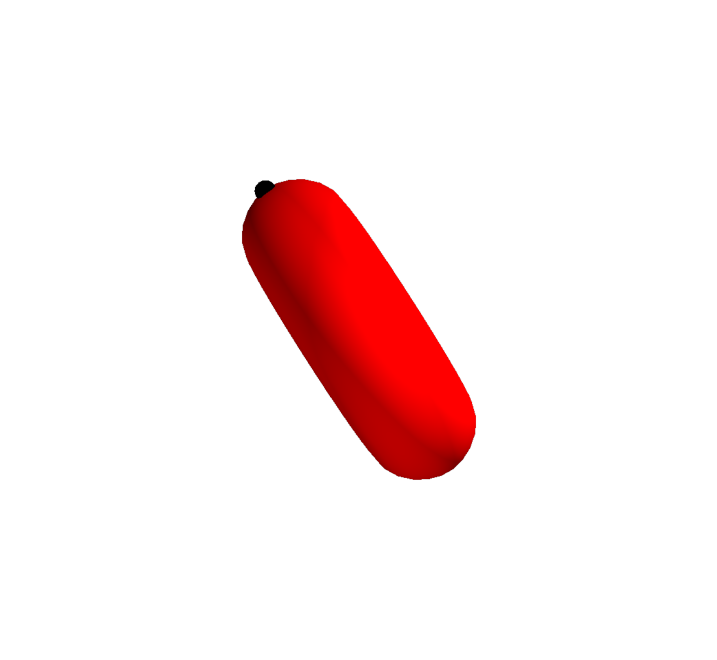
\includegraphics[trim=75 100 75 100, clip, width=\textwidth]{figures/tumble0000.png}}{0.5cm}{0.25cm}\\
        $\dot{\gamma}t = 0$
    \end{minipage}%
    \begin{minipage}{0.2\textwidth}
        \centering
        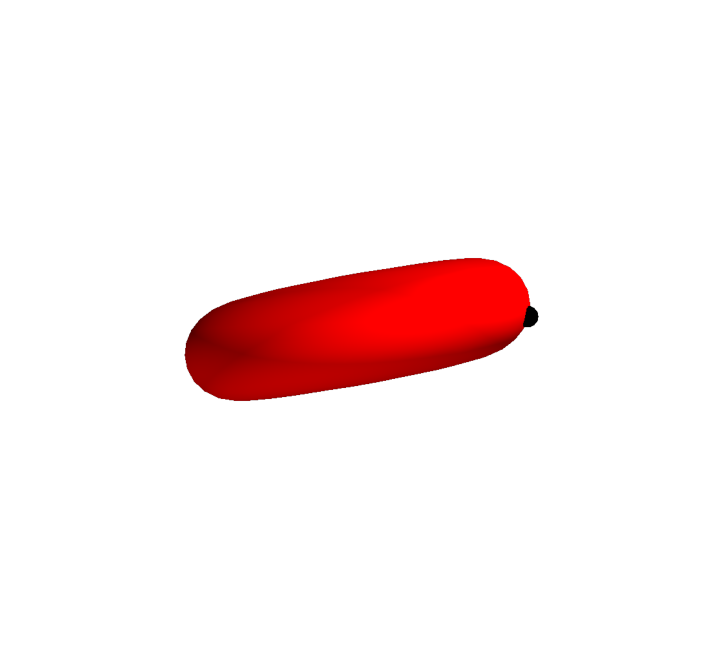
\includegraphics[trim=75 100 75 100, clip, width=\textwidth]{figures/tumble1000.png}\\
        $\dot{\gamma}t = 5$
    \end{minipage}%
    \begin{minipage}{0.2\textwidth}
        \centering
        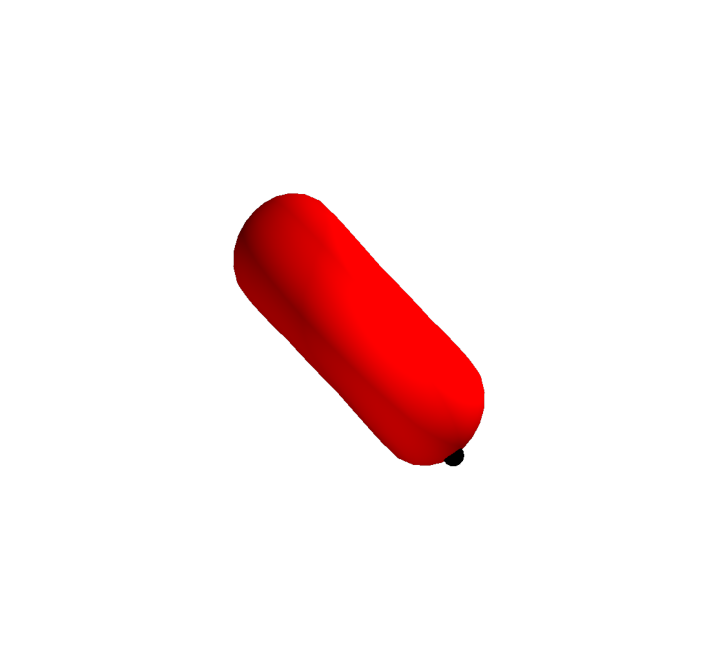
\includegraphics[trim=75 100 75 100, clip, width=\textwidth]{figures/tumble2000.png}\\
        $\dot{\gamma}t = 10$
    \end{minipage}%
    \begin{minipage}{0.2\textwidth}
        \centering
        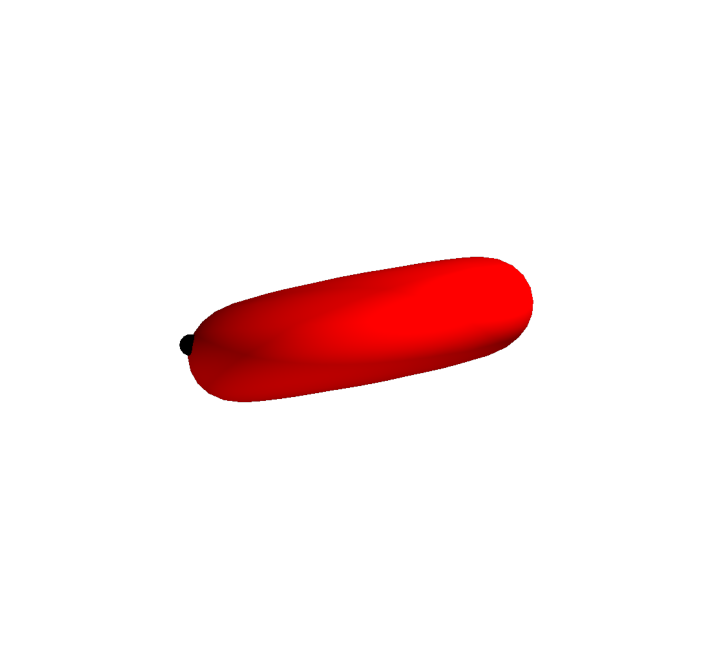
\includegraphics[trim=75 100 75 100, clip, width=\textwidth]{figures/tumble3000.png}\\
        $\dot{\gamma}t = 15$
    \end{minipage}%
    \begin{minipage}{0.2\textwidth}
        \centering
        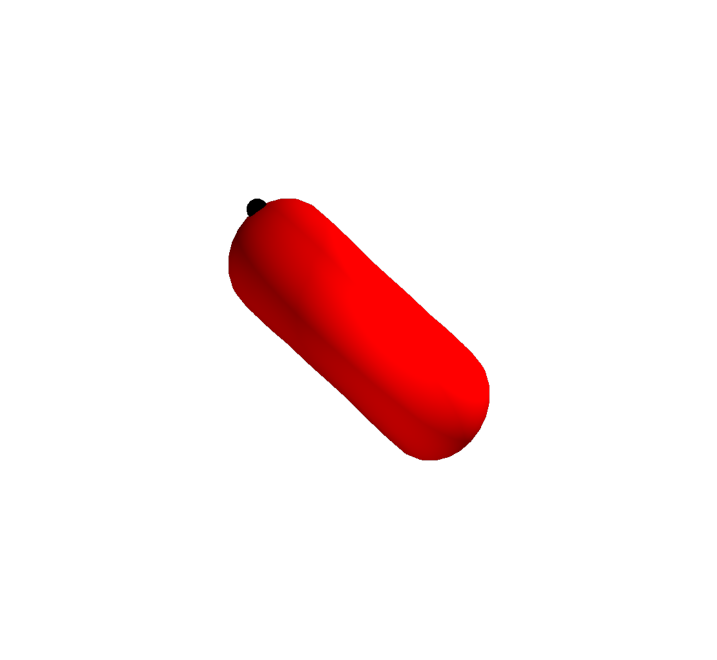
\includegraphics[trim=75 100 75 100, clip, width=\textwidth]{figures/tumble4000.png}\\
        $\dot{\gamma}t = 20$
    \end{minipage}%
    \phantomsubcaption
    \label{fig:tumble}
    \end{subfigure}
    \begin{subfigure}{\textwidth}
    \begin{minipage}{0.2\textwidth}
        \centering
        \topinset{(b)}{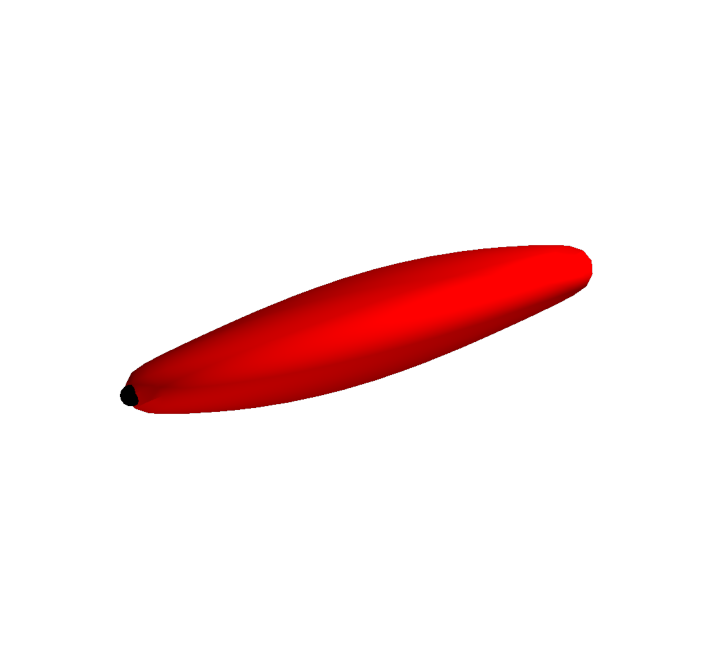
\includegraphics[trim=75 125 75 75, clip, width=\textwidth]{figures/tread0190.png}}{0.5cm}{0.25cm}\\
        $\dot{\gamma}t = 19$
    \end{minipage}%
    \begin{minipage}{0.2\textwidth}
        \centering
        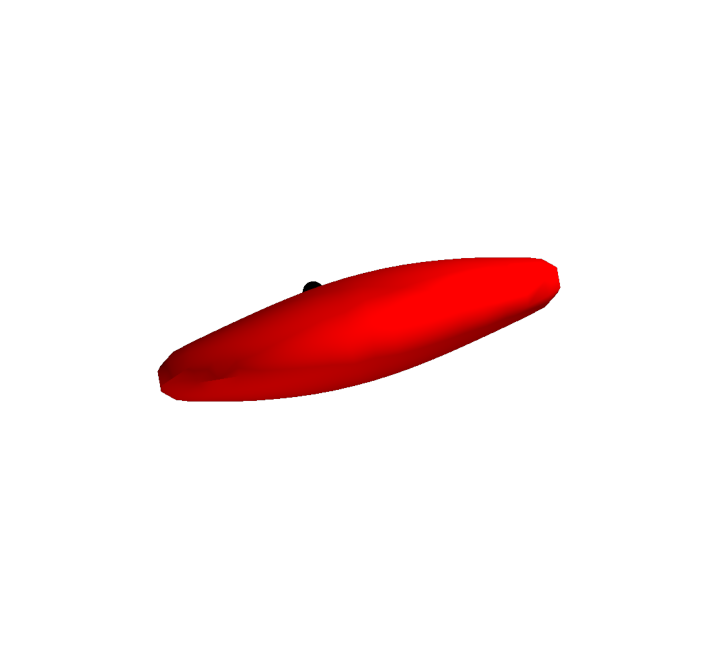
\includegraphics[trim=75 125 75 75, clip, width=\textwidth]{figures/tread0260.png}\\
        $\dot{\gamma}t = 26$
    \end{minipage}%
    \begin{minipage}{0.2\textwidth}
        \centering
        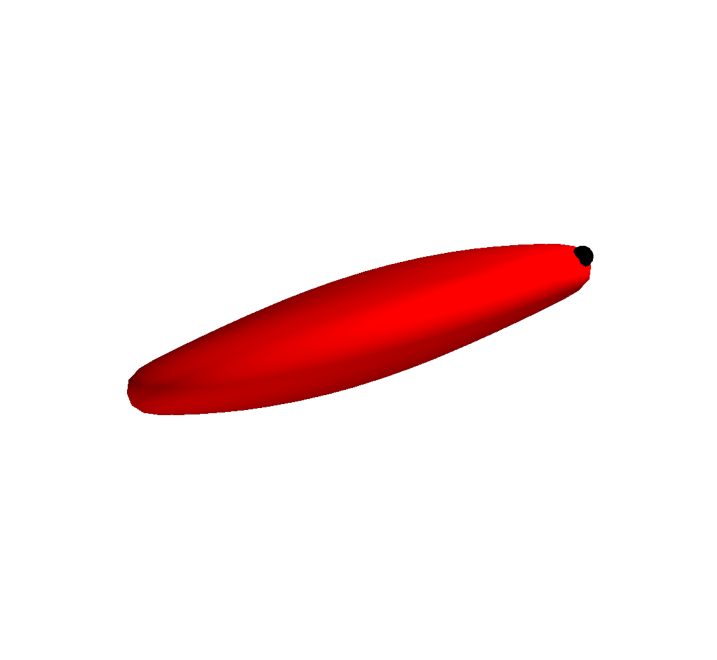
\includegraphics[trim=75 125 75 75, clip, width=\textwidth]{figures/tread0330.png}\\
        $\dot{\gamma}t = 33$
    \end{minipage}%
    \begin{minipage}{0.2\textwidth}
        \centering
        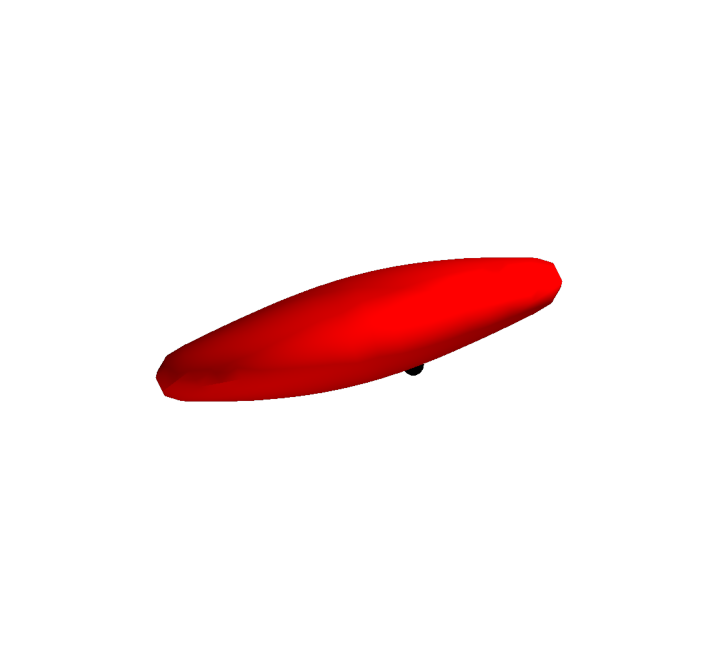
\includegraphics[trim=75 125 75 75, clip, width=\textwidth]{figures/tread0400.png}\\
        $\dot{\gamma}t = 40$
    \end{minipage}%
    \begin{minipage}{0.2\textwidth}
        \centering
        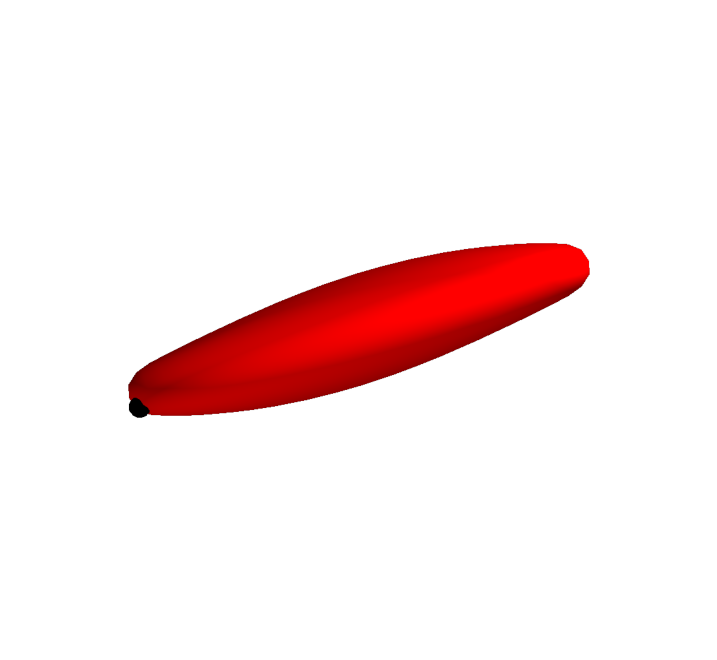
\includegraphics[trim=75 125 75 75, clip, width=\textwidth]{figures/tread0470.png}\\
        $\dot{\gamma}t = 47$
    \end{minipage}%
    \phantomsubcaption
    \label{fig:tread}
    \end{subfigure}
    \caption{%
        Our model RBC exhibits (a) a tumbling behavior under low shear
        ($\dot{\gamma} = 50\si{\per\second}$) conditions and (b) tank-treading under high
        shear ($\dot{\gamma} = 1000\si{\per\second}$) conditions.
    }%
    \label{fig:tumble-tread}
\end{figure}

%RBCs are known to tumble end-over-end under low shear conditions. As shear rates
%increase, the behavior transitions into a regime known as ``tank-treading'', in which
%the cell takes on an elongated shape and the membrane {\XXX} rotates about its interior
%fluid.
%
%We place a single RBC with $\data\cardinality = 625$ and $\sample\cardinality = 2500$
%in a $16\um\times16\um\times16\um$ domain, discretized to have $h = 0.4\um$. We use shear
%rate $\dot{\gamma} = 50\si{\per\second}$ to capture the tumbling dynamics and
%$\dot{\gamma} = 1000\si{\per\second}$ for tank-treading. One period of each is shown in
%Figure~\ref{fig:tumble-tread}.

\subsection{Collision tests}

With whole blood simulation as the ultimate goal, we must ensure that the method can effectively capture cell-cell
interactions. The RBF-IB method has been applied to flow around multiple platelets in an aggregate, but those
cells are kept apart by a network of springs~\cite{Shankar:2015km}. To study the interaction between cells, we
devise a series of tests in which we force two RBCs to collide. The aim is to verify that the cells remain
distinct. Using too few data sites could allow the cells to come too close to one another. The regularization of
$\Dirac_h$ then causes them to be treated as a single unit. Cells that ``fuse'' in this manner are problematic,
generally causing the simulation to end when the cells attempt to separate.

\begin{figure}[tb]
    \centering
    \begin{subfigure}[t]{.25\textwidth}
        \centering
        \topinset{(a)}{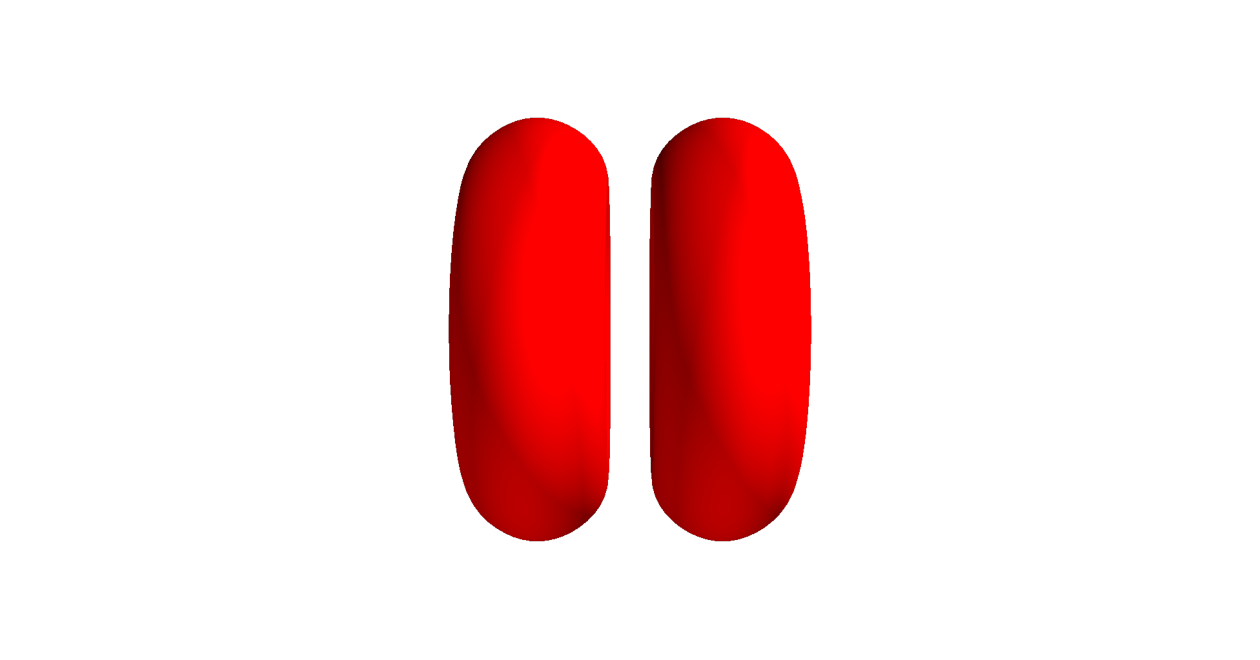
\includegraphics[width=\textwidth]{figures/vvcoll-start.png}}{0.125cm}{0.25cm} \\
        $t = 0\ms$
    \end{subfigure}%
    \begin{subfigure}[t]{.25\textwidth}
        \centering
        \topinset{(b)}{
\includegraphics[width=\textwidth]{figures/vvcoll-end.png}}{0.125cm}{0.25cm} \\
        $t = 1.5\ms$
    \end{subfigure}%
    \begin{subfigure}[t]{.25\textwidth}
        \centering
        \topinset{(c)}{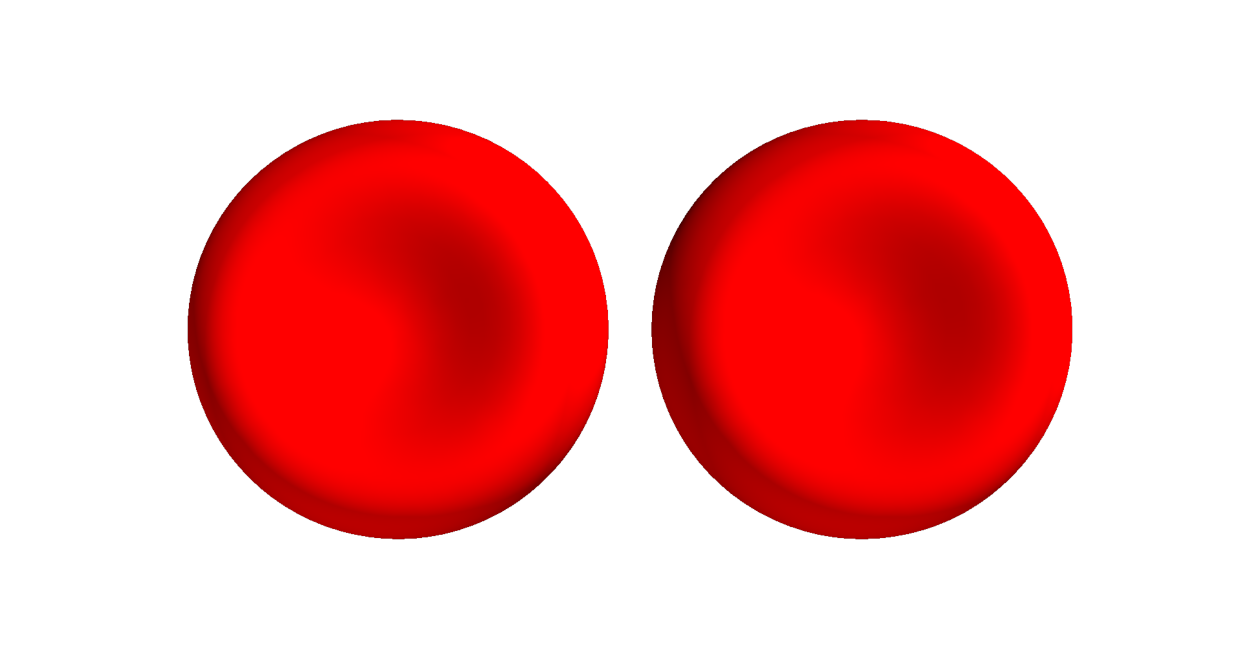
\includegraphics[width=\textwidth]{figures/hhcoll-start.png}}{0.125cm}{0.25cm} \\
        $t = 0\ms$
    \end{subfigure}%
    \begin{subfigure}[t]{.25\textwidth}
        \centering
        \topinset{(d)}{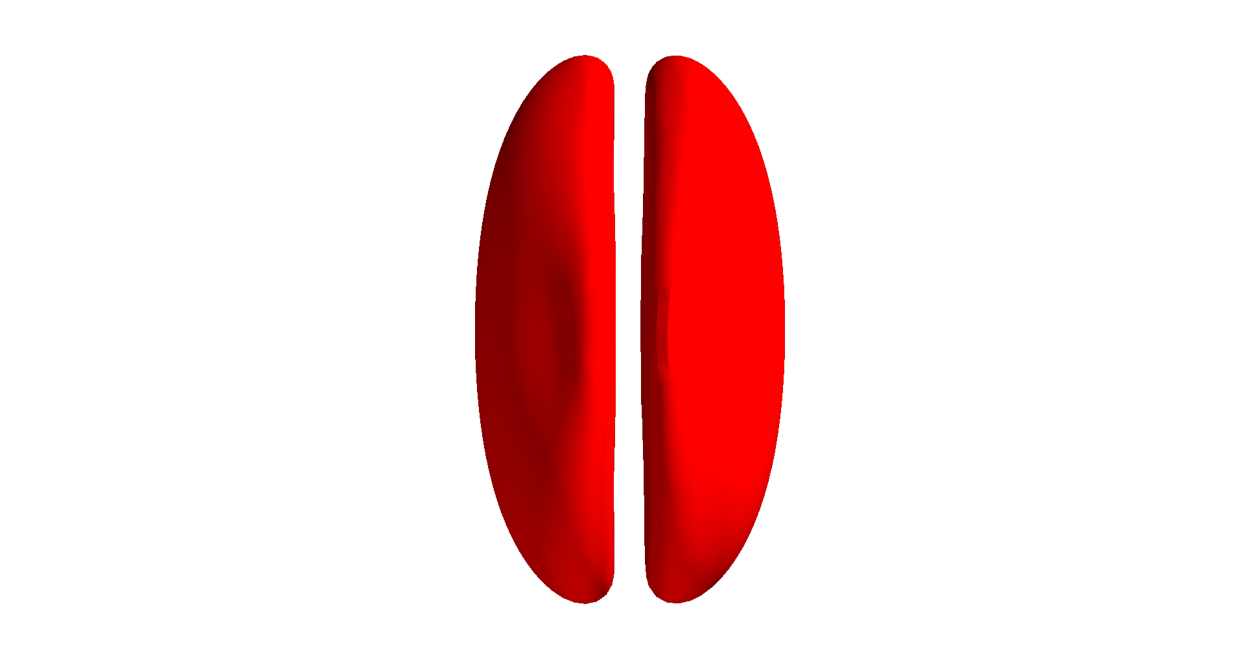
\includegraphics[width=\textwidth]{figures/hhcoll-end.png}}{0.125cm}{0.25cm} \\
        $t = 1.1\ms$
    \end{subfigure}

    \vspace{1em}

    \begin{subfigure}[t]{.25\textwidth}
        \centering
        \topinset{(e)}{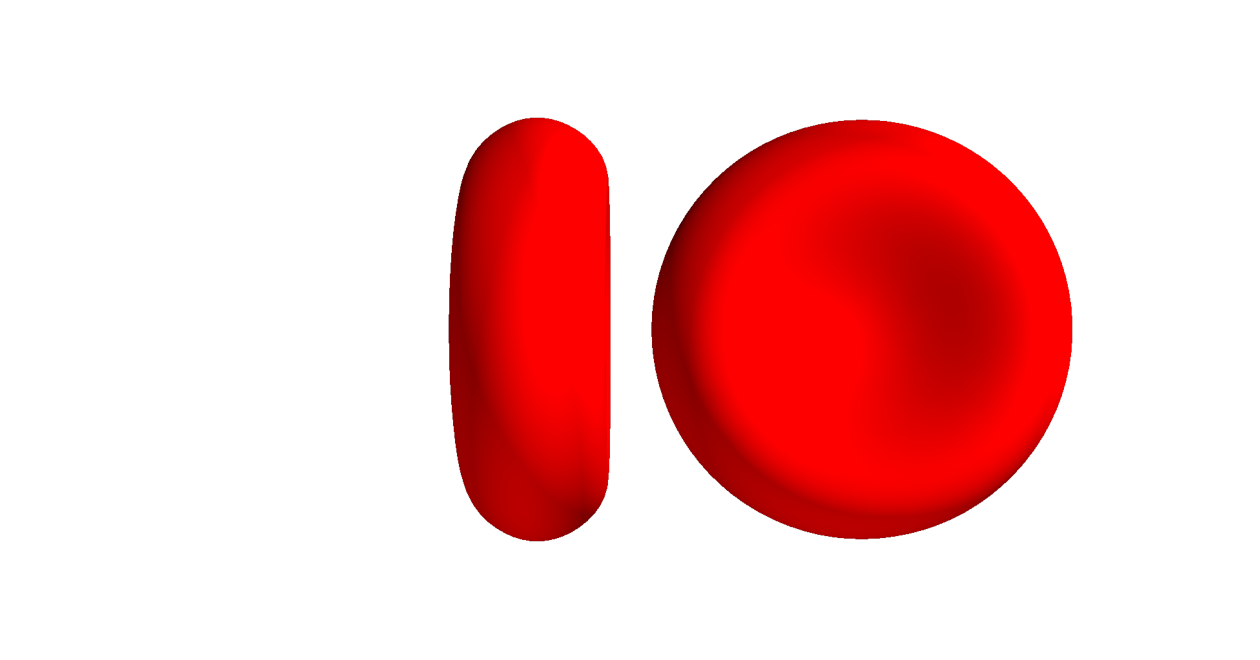
\includegraphics[width=\textwidth]{figures/vhcoll-start.png}}{0.125cm}{0.25cm} \\
        $t = 0\ms$
    \end{subfigure}%
    \begin{subfigure}[t]{.25\textwidth}
        \centering
        \topinset{(f)}{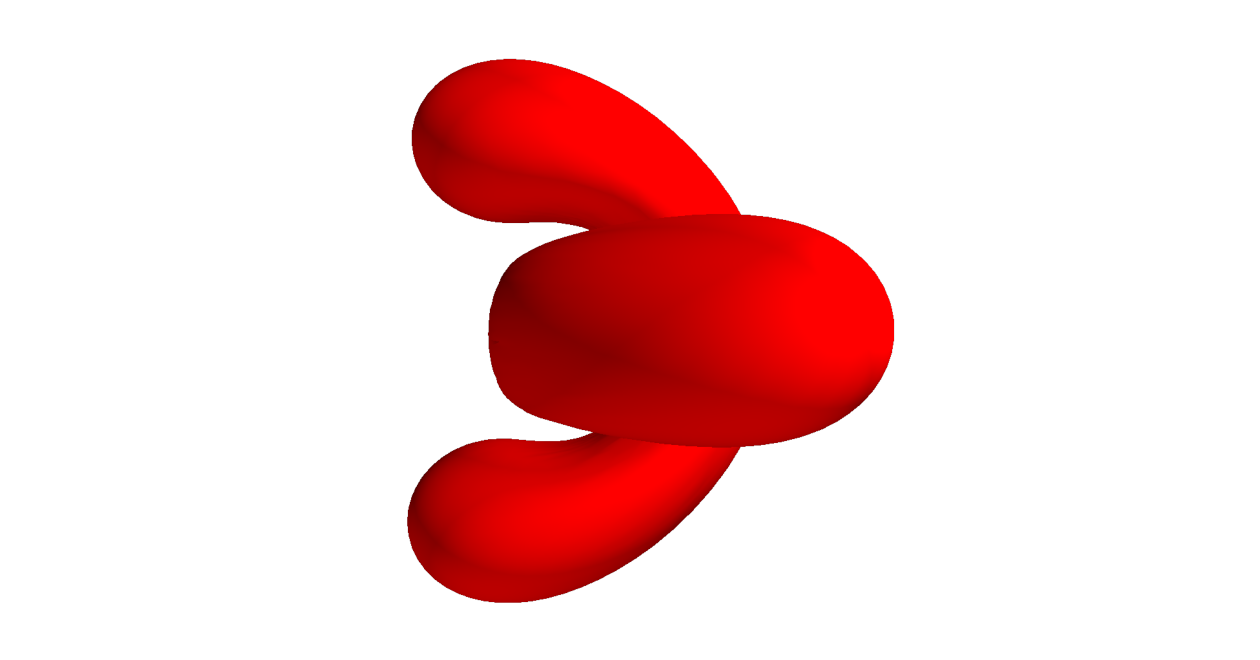
\includegraphics[width=\textwidth]{figures/vhcoll-end.png}}{0.125cm}{0.25cm} \\
        $t = 1.5\ms$
    \end{subfigure}%
    \begin{subfigure}[t]{.25\textwidth}
        \centering
        \topinset{(g)}{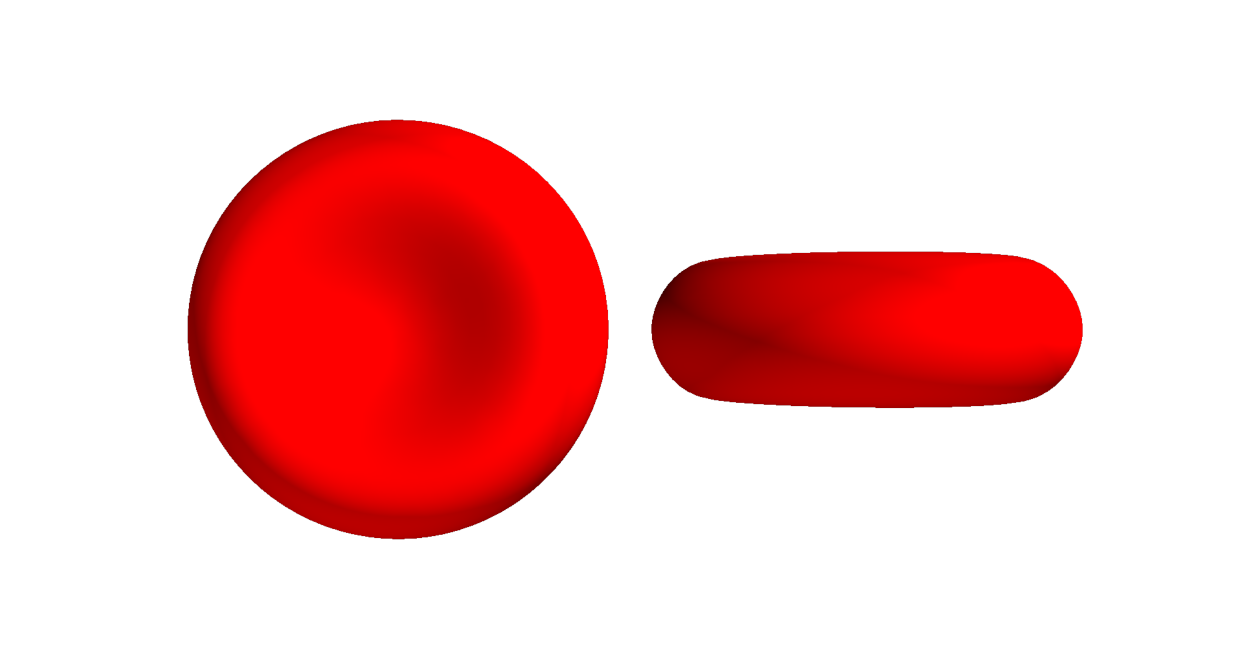
\includegraphics[width=\textwidth]{figures/rhhcoll-start.png}}{0.125cm}{0.25cm} \\
        $t = 0\ms$
    \end{subfigure}%
    \begin{subfigure}[t]{.25\textwidth}
        \centering
        \topinset{(h)}{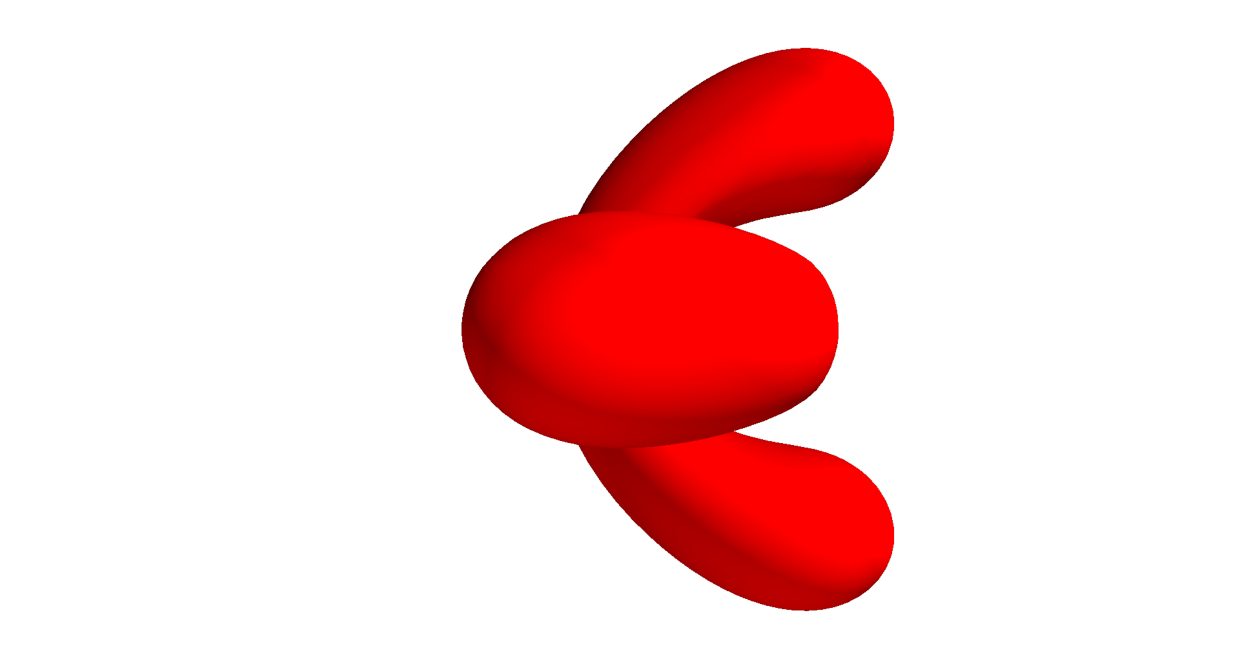
\includegraphics[width=\textwidth]{figures/rhhcoll-end.png}}{0.125cm}{0.25cm} \\
        $t = 1.1\ms$
    \end{subfigure}
    \caption{%
Collision tests between two RBCs. A fictitious force is added to the RBCs to draw them together. (a) and (b) The
RBCs are initially aligned with concavities facing one another. By $1.5\ms$, the cells take on a hemispherical
shape. The concavities in the gap are maintained. Shortly thereafter, asymmetries in the setup lead to the cells
sliding past one other. (c) and (d) The RBCs are initially aligned with their edges facing one another. By
$1.1\ms$, the cells take on a hemispherical shape. The remnants of the concavity can be seen on the left cell in
(d). Shortly thereafter, these cells also slide past one another. (e) and (f) The RBCs are initially aligned with
the edge of one facing a concavity of the other. The cells wrap around each other by $1.5\ms$, taking on a bulbous
banana shape. (g) and (h) The RBCs are initially aligned with their edges facing one another with one of the cells
rotated about the axis $\e_1+\e_3$ by $\pi/2$. By $1.1\ms$, the cells wrap around each other, again taking on the
bulbous banana shape.
    }%
    \label{fig:collisions}
\end{figure}

We continue to use the same physical domain as in the previous two sections, now with $h = 0.2\um$, and place two
RBCs therein, each with $\data\cardinality=2500$ and $\sample\cardinality=10000$. The ratio
$\sample\cardinality/\data\cardinality=4$ is chosen so that sample sites with spacing $h$ means data sites have
spacing $2h$. We believe this to suffice in preventing cells from intersecting, but this is not guaranteed if the
points do not maintain appropriate spacing throughout a simulation. We use the 2-stage RK method with time step
$\timestep = 50\ns$. To interpolate velocities and spread forces, we use the 4-point cosine $\kernel$~%
\cite{Peskin:2002go}. The cells are placed with cell centers on the line $x = z$, $y = 8\um$. They are initially
separated by a gap of $4h = 0.8\um$ between their convex hulls, \latin{i.e.}, ignoring the concavities. Inspired
by Crowl \& Fogelson~\cite{Erickson:2011cf}, we add the fictitious force density
\begin{equation}
    \F_\text{fict} = \pm 0.1\dynpercm\cdot(\e_1+\e_3)/\sqrt{2},
\end{equation}
to each cell, where the sign is chosen so the force points into the gap, to draw the cells together. Success in
these tests implies that this configuration of data and sample sites, the spatial resolution, and the time step
are acceptable for whole blood simulations.

Initial conditions and configurations after a short time are illustrated in \cref{fig:collisions}, where we view
them from above the $x=z$ plane. In each case, the cells move slightly closer together and then undergo
considerable deformation. The data sites are initially approximately $2h$ apart from each other. No problems seem
to arise from this, and in some cases the cells eventually attempt to slide past one another.  We also deduce that
the IB method with the cosine kernel can resolve interactions at a distance of $h$ to $2h$. We consider cells
passing within this threshold to be in contact. Throughout the simulation, the cells remain distinct, and the
simulations end due to extreme forces triggering the stopping condition~\cite{Agresar:1998wv}
\begin{equation}
    \timestep > \frac14\sqrt{\frac{h\rho}{\|\f\|_\infty}}.
\end{equation}
For the remainder of this chapter, we will consider only this arrangement of data and sample sites and this grid
resolution.

\subsection{Whole blood}\label{sec:whole-blood}

In what follows, we consider a $16\um\times12\um\times16\um$ domain with periodic
boundaries in the $x$ and $z$ directions and with Dirichlet boundary conditions in the
$y$ direction. The fluid velocity is initially zero except at the top boundary, where it
moves at $12\mmpersec$. In the absence of cells, the flow tends toward steady Couette
flow with a shear rate of $\shear=1000\persec$. This serves as our model near-wall region
of a blood vessel.

For whole blood simulations, we return to the 4-point B-spline, $B_3$, as the IB kernel.
Because we are limited to very small time steps with either timestepping scheme, we use
backward-forward Euler with $\timestep=50\ns$ to reduce simulation time. We observe
qualitative agreement between these two schemes.  We have already settled on an RBC
discretization in the previous section. We use the same spiral method to discretize the
platelet, but with 900 data and sample sites. Using the same number of sample sites and
data sites aligns more closely with traditional IB methods. We also find that the Bauer
spiral places points more densely along the edge of the platelet, which is helpful in
resolving the large curvatures there. We parametrize the surface of the endothelium over
$(\theta,\,\varphi) \in [0,\,2\pi)^2$ with reference shape
\begin{equation}
    \vec{\hat{X}}_\text{endo}(\theta,\,\varphi) = \left[\begin{array}{c}
            16\um\cdot(\theta/2\pi)  \\
            y(\theta,\,\varphi) \\
            16\um\cdot(\varphi/2\pi)
    \end{array}\right],
\end{equation}
where $y(\theta,\,\varphi)$ depends on the shape under study. The endothelium is
discretized using 16000 points, defined by the spiral
\begin{align*}
    \varphi_i &= 2\pi (i-1)/N, \\
    \theta_i &= \modulo\left(\left\lceil\!\sqrt{N}\mskip\thinmuskip\right\rceil\varphi_i,\,2\pi\right).
\end{align*}
We consider two shapes for the endothelium. The first, $y=1\um$, emulates the flat wall
typically seen in near-wall simulations of RBCs or platelets. The other attempts to
recreate the elongated endothelial cell shape typical of exposure to high-shear
conditions,
\begin{equation*}
    y(\theta,\,\varphi) = 0.75\um + 1\um\cdot\cos^2(\theta-\varphi)\sin^2(\varphi/2).
\end{equation*}
The bumps have a prominence of $1\um$. The endothelial surface is raised by $0.75\um$ to
avoid it interacting with the domain boundary. The positions of the surface are chosen to
maintain a fixed hematocrit of approximately 34\% for both endothelial shapes.

As a preliminary validation of the platelet model and to establish baseline platelet
motion, we consider two platelets along a flat wall. They are placed parallel to the wall
at distances of $0.3\um$ and $0.5\um$. The domain does not contain any RBCs. At a
distance of $0.3\um$, the platelet is expected to ``wobble'', in which the platelet tilts
slightly upward and downward, periodically~\cite{King:2005fv}. On the other hand, the
platelet initially $0.5\um$ from the wall should tumble end-over-end $0.5\um$. We observe
wobbling at a frequency of approximately $10\persec$ and tumbling with a frequency of
approximately $30\persec$. We also note that the edge of the tumbling platelet remains
pointed towards the wall for only 3--$4\ms$.

\subsubsection{Initialization}\label{sec:blood-init}

We begin by assuming that the platelets have already been marginated by the RBCs. We
think of the domain as having three layers with the endothelium at the bottom, RBCs on
top, and platelets in between. We begin by settling the endothelium and RBCs before
placing platelets.

In addition to the endothelium, we place 2 rows of 4 RBCs, each in their reference
configuration, in the domain with the RBCs' centers of mass on the plane $y=6\um$.
Because the domain is not wide enough to accommodate two reference RBCs alongside one
another, the cells are staggered by $2\um$. These locations are then randomly translated
and rotated while maintaining a distance of at least $2h$ between cells.

Before placing any platelets in the domain, we allow the flow to develop with only the
endothelium and RBCs. We allow the initialization to continue until at least $17\ms$,
which is approximately when the first RBC overtakes its neighbor. From here, we choose a
series of times, sampled from a Poisson distribution to be approximately $3\ms$ apart, at
which to begin simulations with platelets.

The RBCs for each of the chosen starting configurations are considerably and
unpredictably deformed and have left a space of a few microns above the endothelium
in which we place platelets. To find reasonable starting orientations for the platelets,
we randomly choose points on the endothelium and one on each platelet surface. Each of
the simulations in the upcoming sections contains two platelets, so we choose two points
on the endothelium that are at least $3.9\um$, a platelet diameter plus $4h$, apart. The
resulting platelet are spaced far enough apart as to not intersect. We compute normal
vectors on the surfaces of the endothelium and platelets at these points. The platelets
are oriented so that the normal emanating from the platelet opposes the normal at the
corresponding point on the endothelium. The platelet is then placed so its chosen surface
point is separated from the endothelium point by a random distance between $0.3\um$ and
$1\um$. If the generated orientation does not pass within $0.4\um$ of an RBC, the
platelet is accepted. Otherwise, we try again with a different platelet point. This
algorithm typically succeeds within 2 attempts.

This initialization process is performed once for each endothelial configuration and we
take the first four acceptable initial configurations for each. In the following section,
we present behaviors found in these simulations. As a point of comparison, we also
consider the initial configurations for the bumpy wall with the RBCs removed from the
domain.


\subsubsection{Characterization of flow and cell behaviors}

In this section, we catalog the differences in the flow between whole blood along a bumpy
and flat wall, and between flow along a bumpy wall with and without RBCs. We aim to
compare the interactions platelets have with RBCs and the endothelium for these test
cases.
%We begin with the expected behaviors before moving on to remarkable ones.

\begin{figure}[tp!]
    \centering
    \begin{tikzpicture}[spy using outlines={rectangle, magnification=3,connect spies}]
        \begin{axis}[
                axis lines=center,
                xmin=0,
                xmax=12.5,
                ymin=0,
                ymax=12.5,
                ylabel={$y$ ($\um$)},
                xlabel={fluid speed ($\mmpersec$)},
                xlabel near ticks,
                ylabel near ticks,
                legend pos=south east,
                legend style={draw=none}
            ]
            \addplot[color=tol/contrast/red, very thick, x filter/.code={\pgfmathparse{\pgfmathresult*10}\pgfmathresult}] table [x index=1, y index=0] {rpefast1.prof.dat};
            \addlegendentry{\cmark~bumps\hspace{0.5em}\cmark~RBCs};
            \addplot[color=tol/contrast/blue, very thick, x filter/.code={\pgfmathparse{\pgfmathresult*10}\pgfmathresult}] table [x index=1, y index=0] {rpeflat1.prof.dat};
            \addlegendentry{\xmark~bumps\hspace{0.5em}\cmark~RBCs};
            \addplot[color=tol/contrast/yellow, very thick, x filter/.code={\pgfmathparse{\pgfmathresult*10}\pgfmathresult}] table [x index=1, y index=0] {pefast1.prof.dat};
            \addlegendentry{\cmark~bumps\hspace{0.5em}\xmark~RBCs};

            \coordinate (spypoint) at (axis cs: 0.5, 1);
            \coordinate (spyviewer) at (axis cs: 2.5, 10);
            \spy[width=2cm,height=2cm] on (spypoint) in node [fill=white] at (spyviewer);
        \end{axis}
    \end{tikzpicture}
    \caption[A comparison of fluid velocity profiles]{%
Time- and space-averaged fluid velocity profiles for each of the test cases.
%The F\r{a}hr{\ae}us-Lindqvist effect is clearly evident when RBCs are included.
The inclusion of RBCs (red and blue curves) causes the region inhabited by platelets,
1--$4\um$, to experience a higher shear rate than it would without RBCs (yellow curve).
    }\label{fig:flow-profiles}
\end{figure}

Flow profiles are shown in Figure~\ref{fig:flow-profiles}. The most notable difference
among the three flow profiles is the nearly Couette flow when RBCs are absent. The only
distinction between this and Couette flow is the smoother transition at the wall, due to
the bumps. This is also the distinguishing feature between the profiles corresponding to
bumpy and flat walls in the presence of RBCs. The smooth transition from the bumps
results in marginally slower flow speeds throughout the domain, compared to the flat
wall. The inclusion of RBCs causes the bends in the red and blue curves around $y = 3\um$
and $y = 9\um$. Platelets inhabit the region between $y=1$ and $3\um$. In simulations
featuring RBCs, the platelets experience higher shear rates than those without RBCs where
there is a reduction in apparent viscosity in the RBC-free layer. This is a consequence
of the F\r{a}hr{\ae}us effect. In pressure-driven flow through a tube, we expect
approximately parabolic flow.  The bend near $y = 9\um$ is therefore nonphysical and
arises from satisfying boundary conditions at the top boundary. However, the increased
shear rate in the region between $y=9$ and $12\um$ seems to be useful in deterring RBCs
from approaching the upper boundary. An exclusionary region of just 1--$2\um$ along the
top boundary increases the effective hematocrit to 37--41\%. Furthermore, the reduced
shear rate in the region containing RBCs results in slower tank-treading compared to a
dilute suspension of RBCs, with one period now lasting approximately $40\ms$.

RBCs are effective at preventing the platelets from moving too far from the endothelium.
The furthest observed distance from the endothelium any platelet takes is just under
$1.5\um$. Likewise, RBCs infrequently enter the cell-free layer, with some notable
exceptions, discussed below. We do not observe any platelet wobbling. Instead, platelets
transiently follow the curve of the bumpy walls, tilt down into the valleys between
bumps, and tumble. Nothing suggests that bumps in the surface of the endothelium alone
can sequester platelets, nor do we directly observe stagnation zones.

\begin{figure}[th!]
    \begin{subfigure}[t]{0.5\textwidth}
        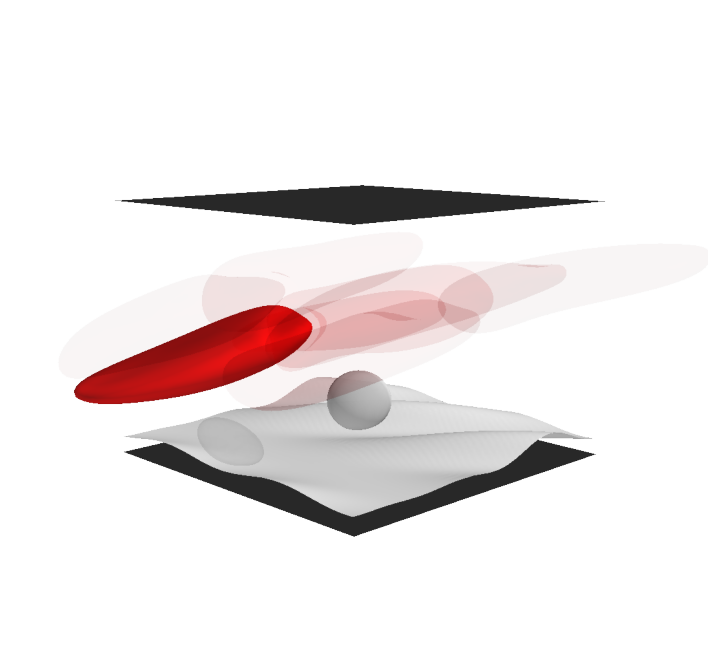
\includegraphics[trim=50 75 50 125, clip, width=\textwidth]{figures/unicycle1.png}
        \subcaption{$t = 46\ms$}
    \end{subfigure}%
    \begin{subfigure}[t]{0.5\textwidth}
        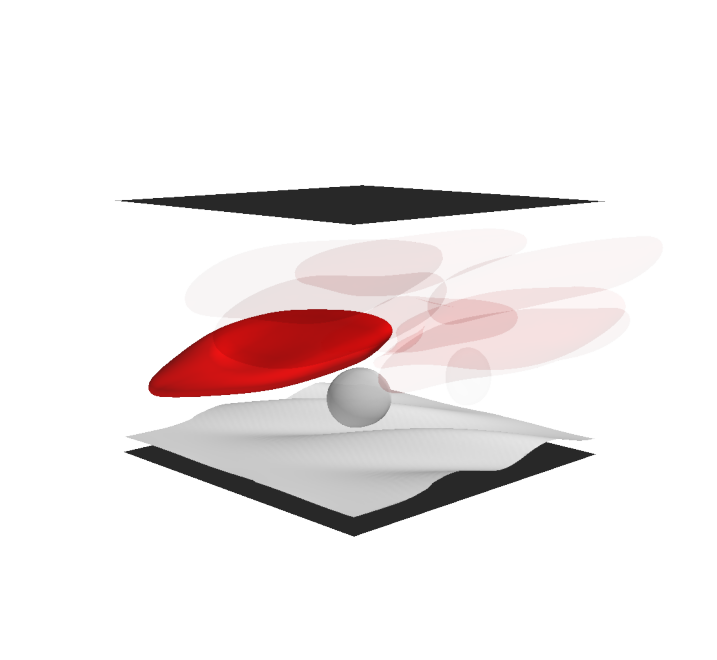
\includegraphics[trim=50 75 50 125, clip, width=\textwidth]{figures/unicycle2.png}
        \subcaption{$t = 48\ms$}
    \end{subfigure}

    \vspace{11pt}

    \begin{subfigure}[t]{0.5\textwidth}
        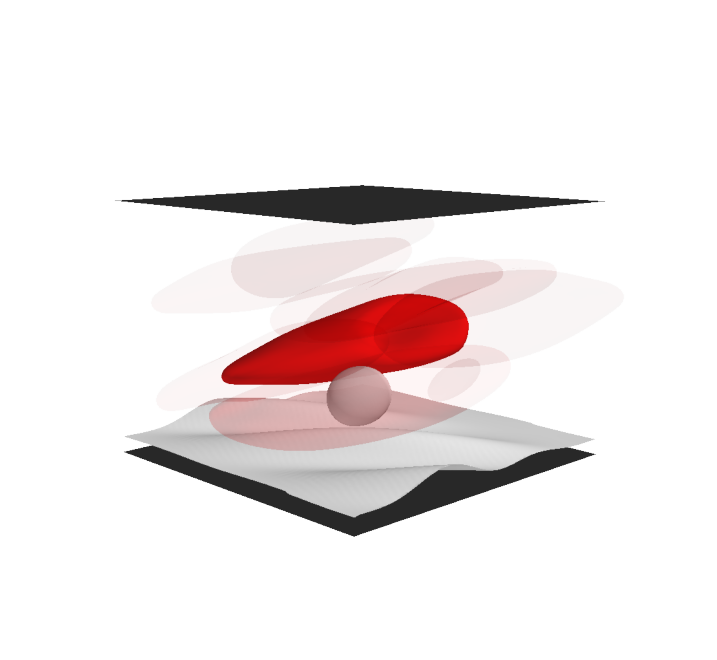
\includegraphics[trim=50 75 50 125, clip, width=\textwidth]{figures/unicycle3.png}%
        \subcaption{$t = 50\ms$}
    \end{subfigure}%
    \begin{subfigure}[t]{0.5\textwidth}
        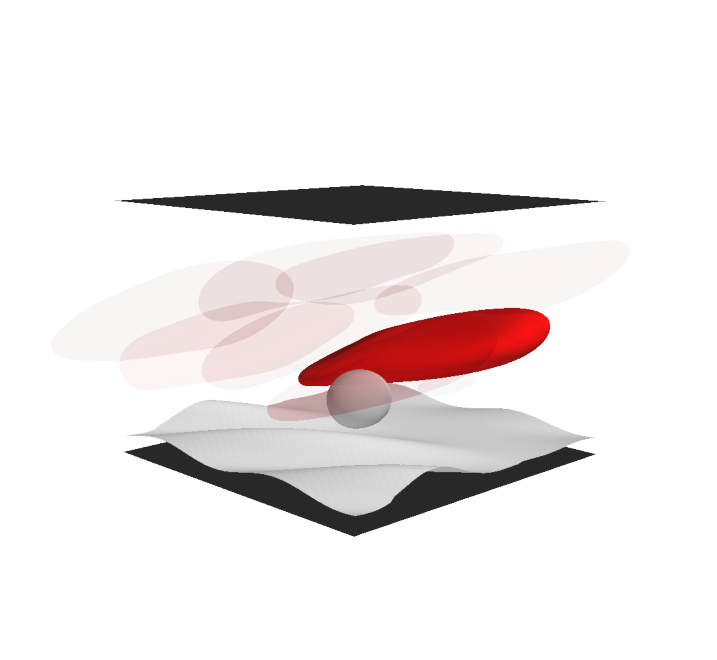
\includegraphics[trim=50 75 50 125, clip, width=\textwidth]{figures/unicycle4.png}%
        \subcaption{$t = 52\ms$}
    \end{subfigure}

    \vspace{11pt}

    \begin{subfigure}[t]{\textwidth}
        \begin{tikzpicture}
            \begin{axis}[
                width=\textwidth,
                height=2in,
                axis lines=center,
                xmin=8.5,
                xmax=61.5,
                ymin=0,
                ymax=0.95,
                ylabel={distance ($\um$)},
                xlabel={time ($\ms$)},
                xlabel near ticks,
                ylabel near ticks
            ]
                \addplot[color=tol/vibrant/magenta, very thick] table [x index=0, y index=6] {rpefast0.dat};
                \addplot[no marks, color=black, dashed] coordinates {(8.5, 0.4)
                                      (61.5, 0.4)};
                \path[name path=axis] (axis cs: 8.5, 0) -- (axis cs: 61.5, 0);
                \addplot[opacity=0, name path=unicycle] table [x index=0, y index=4] {rpefast0.dat};
                \addplot[fill=tol/vibrant/magenta, fill opacity=0.2] fill between[of=unicycle and axis];

                \node at (axis cs: 10.5, 0.9) {(e)};
            \end{axis}
        \end{tikzpicture}
    \end{subfigure}
    \caption[Platelet unicycling behavior]{%
(a)--(d) Snapshots of a platelet rolling on its edge (``unicycling'') with RBCs, one
translucent, flanking either side. The camera tracks the opaque platelet. It's motion is
indicated by the endothelium moving from right to left. (e) The distance between
the platelet and the endothelium. The shaded region indicates that the orientation of the
platelet's short axis is within $45^\circ$ of the vorticity direction.  The black dashed
line indicates $2h$ and is the maximum distance that might be considered contact with the
endothelium. See~\ref{sec:supp} for a video corresponding to this simulation.
    }\label{fig:unicycle}
\end{figure}

Bumpy endothelium simulations without RBCs mimic those with a flat wall; platelets move
away from the wall to a point where they are free to tumble. Unsurprisingly, we observe
platelet tumbling for both flat and bumpy walls with RBCs as well. In Stokes-like flow, a
rigid platelet would tumble faster in flow with a higher shear rate. We might therefore
expect the platelet to tumble faster with RBCs. However, RBCs can significantly disturb
the fluid around a platelet, speeding up its motion, slowing it down, or preventing a
tumble altogether.

We observe platelets rolling in the flow direction along their edge. Because the
platelet in this arrangement is aligned vertically, part of the edge stays in
near-contact with the endothelium while the opposite edge extends into the region
occupied by RBCs.  Contact with RBCs is frequent. These contacts can have a destabilizing
effect, but may also prolong the rolling. Figure~\ref{fig:unicycle}(a)--(d) consists of a
series of snapshots illustrating the behavior. The platelet in this case is flanked by
two RBCs, so it does not have the space to topple over until the RBCs pass a few
milliseconds later.

While Figure~\ref{fig:unicycle} shows this phenomenon on a bumpy wall, it can also occur
above a flat wall. We first observed this motion with a flat wall, and there it lasted
over $40\ms$. The motion was maintained, in part, by an RBC that rode along the top of
the platelet, partially enveloping that platelet. We say that a platelet rolling on its
edge is \term{unicycling}. Figure~\ref{fig:unicycle}(e) illustrates that the platelet
spends more time in contact or near-contact with the endothelium while unicycling
compared to the tumbles near $t=16\ms$ and $t=29\ms$. Though RBCs seem to control the
duration of the unicycling, they are not strictly necessary for unicycling to occur. In
tests with a bumpy wall without RBCs, unicycling is initiated when a platelet rolls
sideways, relative to the flow direction, off of a bump. Without RBCs, the platelet
maintains the vertical alignment for a majority of the simulation thereafter. However,
without frequent interaction with RBCs, the platelet in these simulations move away from
the wall.  Moreover, while we have not observed it directly, we expect that a lone
platelet traveling over a flat wall would also exhibit unicycling, given the right
initial orientation.

\begin{figure}[th!]
    \begin{subfigure}[t]{0.5\textwidth}
        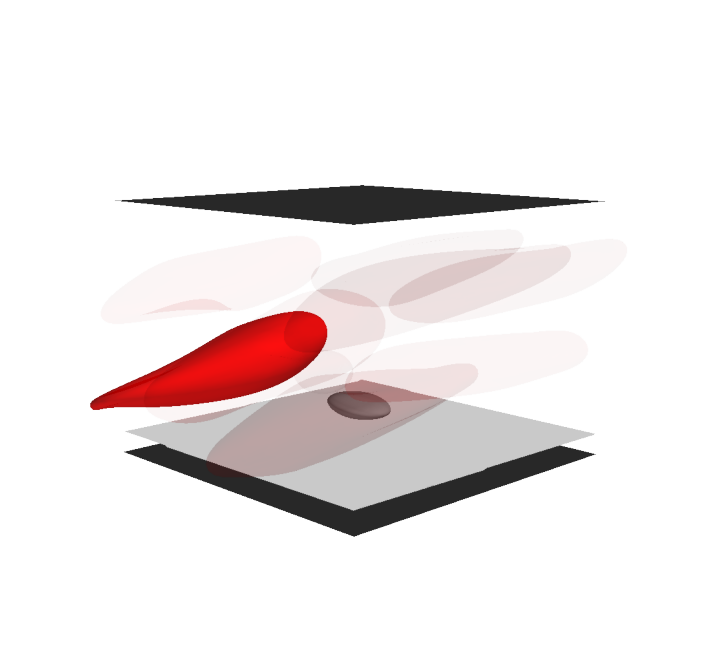
\includegraphics[trim=50 75 50 125, clip, width=\textwidth]{figures/flyover460.png}%
        \subcaption{$t = 46.0\ms$}
    \end{subfigure}%
    \begin{subfigure}[t]{0.5\textwidth}
        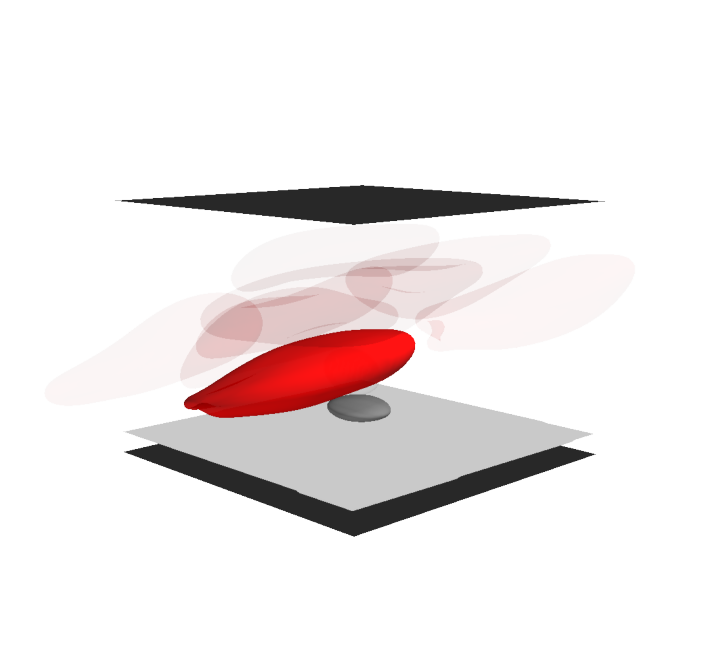
\includegraphics[trim=50 75 50 125, clip, width=\textwidth]{figures/flyover495.png}
        \subcaption{$t = 49.5\ms$}
    \end{subfigure}

    \vspace{11pt}

    \begin{subfigure}[t]{0.5\textwidth}
        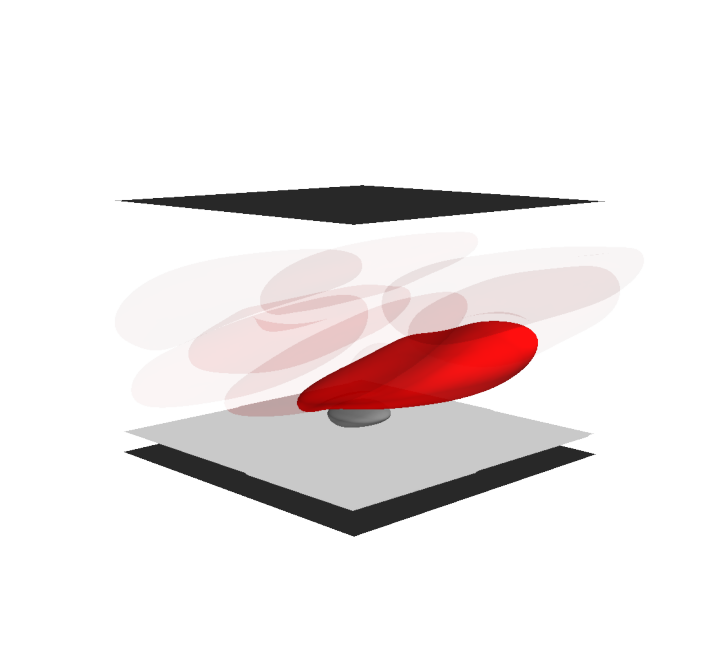
\includegraphics[trim=50 75 50 125, clip, width=\textwidth]{figures/flyover530.png}%
        \subcaption{$t = 53.0\ms$}
    \end{subfigure}%
    \begin{subfigure}[t]{0.5\textwidth}
        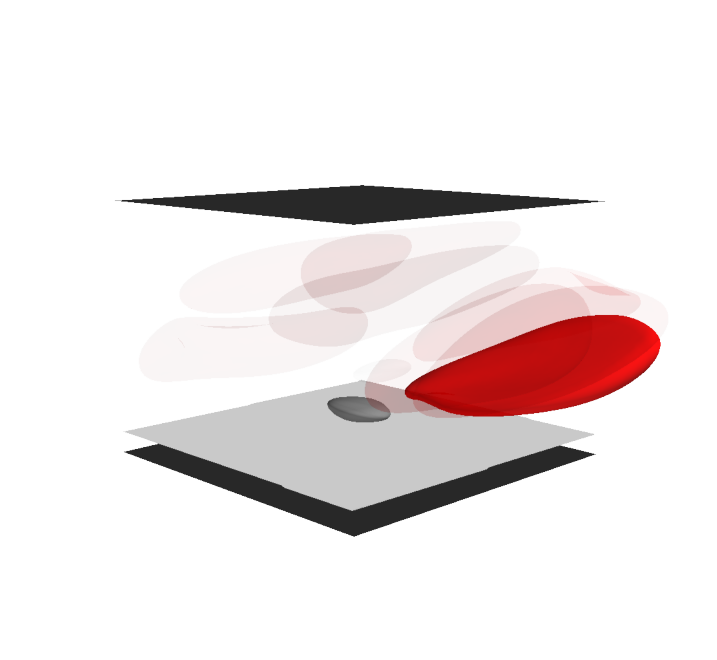
\includegraphics[trim=50 75 50 125, clip, width=\textwidth]{figures/flyover565.png}%
        \subcaption{$t = 56.5\ms$}
    \end{subfigure}

    \vspace{11pt}

    \begin{subfigure}[t]{\textwidth}
        \begin{tikzpicture}
            \begin{axis}[
                width=\textwidth,
                height=2in,
                axis lines=center,
                xmin=8.5,
                xmax=61.5,
                ymin=0,
                ymax=3.25,
                ylabel={velocity ($\mmpersec$)},
                xlabel={time ($\ms$)},
                xlabel near ticks,
                ylabel near ticks
            ]
                \addplot[color=tol/vibrant/magenta, very thick] table [x index=0, y index=3] {rpeflat3.vel.dat};
                \path[name path=axis] (axis cs: 8.5, 0) -- (axis cs: 61.5, 0);
                \addplot[opacity=0, name path=deformed, y filter/.code={\pgfmathparse{#1*3}\pgfmathresult}] table [x index=0, y index=4] {rpeflat3.vel.dat};
                \addplot[fill=tol/vibrant/magenta, fill opacity=0.2] fill between[of=deformed and axis];

                \node at (axis cs: 10.5, 3) {(e)};
            \end{axis}
        \end{tikzpicture}
    \end{subfigure}
    \caption[RBC-mediated platelet-endothelial collision]{%
(a)--(d) Snapshots of RBC-mediated collision between a platelet and the endothelium. (a)
The platelet attempts to tumble. (b)--(c) An RBC comes into proximity with the platelet,
deflects to avoid the platelet, and pushes the platelet into the endothelium, thereby
preventing the platelet from tumbling. (d) The platelet is free to tumble again. (e) The
minimum velocity on the surface of the platelet. The shaded region indicates that the
relative change in aspect ratio exceeds 4\%. See~\ref{sec:supp} for a video corresponding
to this simulation.
    }\label{fig:rbc-plt-endo-collision}
\end{figure}

We notice that in simulations with a bumpy endothelium, platelets will collide with the
bumps. This tends to occur while the platelet is tumbling, and the edge of the platelet
makes contact with the endothelium. This interaction is characterized by deformations
that flatten the edge of the platelet and a \midtilde5\% relative
change in the aspect ratio of the platelet. However, the collision need not occur along
the edge of the platelet, nor, indeed, against a bump in the endothelium. Similar
collisions occur in the case of a flat wall, suggesting that RBCs mediate this behavior.
A clear case of this is illustrated in Figure~\ref{fig:rbc-plt-endo-collision}(a)--(d).
We also note that the few milliseconds preceding the unicycling in Figure~%
\ref{fig:unicycle} correspond to a collision with the wall, showing that this is yet
another trigger for unicycling to occur.

Because the platelet comes into contact with the endothelium, or nearly does so, the
platelet slows along the area of contact. Figure~\ref{fig:rbc-plt-endo-collision}(e)
shows the correlation between the relative change in aspect ratio and the reduction in
minimum platelet surface velocity. Though the aspect ratio of the platelet changes
somewhat while normally tumbling, changes of this magnitude seem to always correspond to
interactions with the endothelium. Collisions with the RBC, for example, result primarily
in deformation of the RBC and deflection of the platelet, which is otherwise relatively
unperturbed.


%PoC that the idea may work:
%\begin{itemize}
%    \item Flat vs elongated at $1000\si{\per\second}$
%    \begin{itemize}
%        \item PLTs + flat wall, no RBCs
%        \item PLTs + flat wall + rbcs --- $\times 4$, different starts
%        \item PLTs + perturbed wall(s) --- $\times 4$, different starts
%    \end{itemize}
%    \item Cobblestone wall
%\end{itemize}

%Random start algo:
%\begin{enumerate}
%    \item Pick $t^n = t^{n-1} + T\ms$, $t^0 = 16\ms$ and $T$ sampled from $\text{Poisson}(3)$. RBCs only start overtaking one another around 16--$19\ms$
%    \item At time $t^n$, $n \ge 1$,
%        \begin{enumerate}
%            \item Pick random endo + PLT points twice, endo points separated by $3.9\um = \text{PLT radius} + 4h$
%            \item compute $\n_\text{endo}$ and $\n_\text{plt}$ at those points
%            \item pick random distance $r$ between $0.3\um$ and $1\um$ twice
%            \item rotate PLTs so $\n_\text{endo} = -\n_\text{plt}$ and the end and plt points are $r$ apart. 
%            \item check that PLT does not get too close to other endo points or RBCs.
%                Favors PLTs oriented at an intermediate angle: more likely to choose points near edge, but they generate a sharp angle, which typically leads to intersection with RBCs.
%            \item otherwise, repeat up 100 times, then give up for this time step
%        \end{enumerate}
%    \item Start simulations at first 4 successful times with added PLTs
%\end{enumerate}
